%!TEX root = ../main.tex
\chapterimage{chapter_head/1_Afterclasse.jpg} 
\chapter{Afterclasse}
\label{ch:afterclasse}
\section{A revision website}
\href{https://www.afterclasse.fr}{Afterclasse.fr} is a revision website released in 2015 by Lelivrescolaire.fr, a French EdTech company (section~\ref{sec:lls}). While most of the educational content on \href{https://www.lelivrescolaire.fr}{Lelivrescolaire.fr} were thought and designed to be used by teachers with their students (in class or at home), Afterclasse is a platform which is designed directly for students to work independently after classroom hours. 

The content covers the official program of the French Education Nationale ministry for middle school - from 11 to 15 years old with the corresponding grades \emph{6ème 5ème 4ème 3ème} - and high school- from 15 to 18 years old with the grades \emph{2nde 1ère Terminale}. In each grade, there are several subjects: French, Mathematics, History and Geography, Physics and Chemistry, Natural Science, Sociology and Economics, English, Spanish, and Philosophy. 

\begin{figure*}[!ht]
\centering
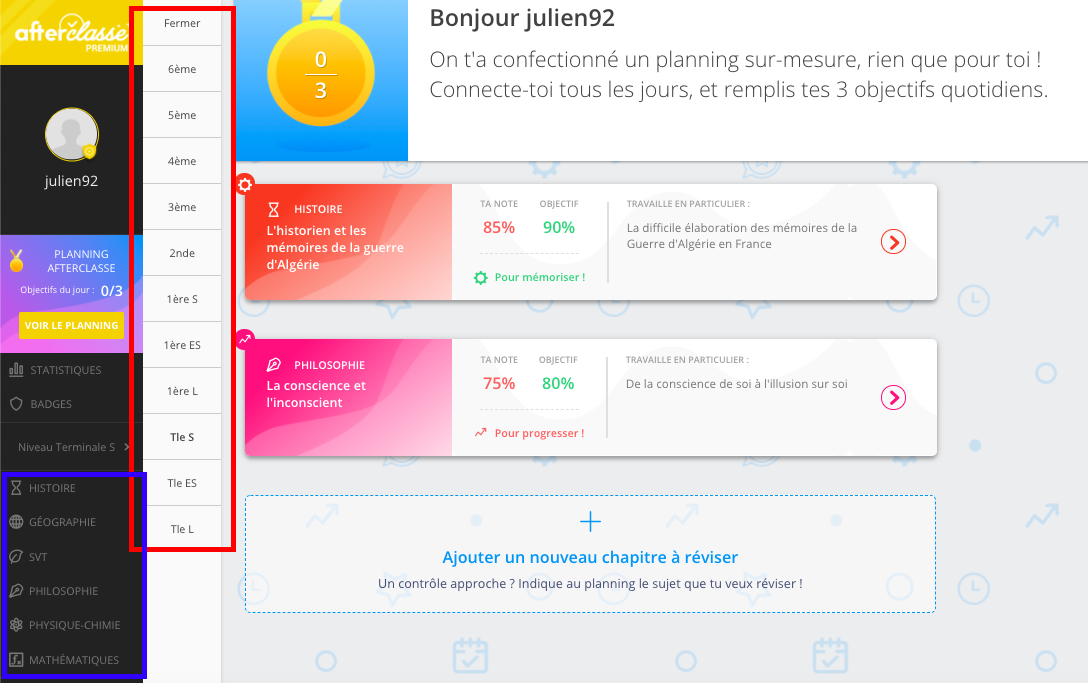
\includegraphics[clip, width= \textwidth]{1literature/fig/afterclasse.png}
\caption{Grades (Red rectangle) and Subjects (Blue rectangle). }
\label{fig:afterclasse}
\end{figure*}

For a given grade, the content of a subject is divided into chapters.  Each chapter is associated with a revision sheet and a self-assessment mode. The revision sheet gathers the main information about the chapter: a lesson plan, definitions, dates, biography of the main characters or authors, etc.

\section{Exercises: format and data}
In the self-assessment mode, the exercises are given sequentially to students. For each chapter, there are roughly one hundred different exercises. An exercise session contains few ($\sim 8$) exercises. At the end of the session, statistics about the session are displayed to the user, and s/he can choose to restart a new session. 

% Exercise session of 20 answers
Each exercise is associated with a topic, a difficulty level, and a type. A topic is a subdivision of a chapter. It usually corresponds to a section of the lesson plan. There are two to four topics for each chapter. There are three levels of difficulty in the course. The easy questions are direct applications from the course or involve prerequisite knowledge from the previous chapters. The medium questions are the core of the course. The difficult questions are either complex exercises either questions which involve knowledge slightly beyond the scope of the course. Notice that the difficulty is tagged by a teacher. It does not necessarily quantify the fraction of students which had succeeded it. Indeed, there are questions that might be easy to answer but involve complex knowledge. There are 7 types of exercises: multiple choice (Figure~\ref{fig:qcm}), single choice (Figure~\ref{fig:qcu}), box (Figure~\ref{fig:box}), link ( Figure~\ref{fig:link}), timeline (Figure~\ref{fig:timeline}), and input (Figure~\ref{fig:input}).  

\begin{figure*}[!ht]
\centering
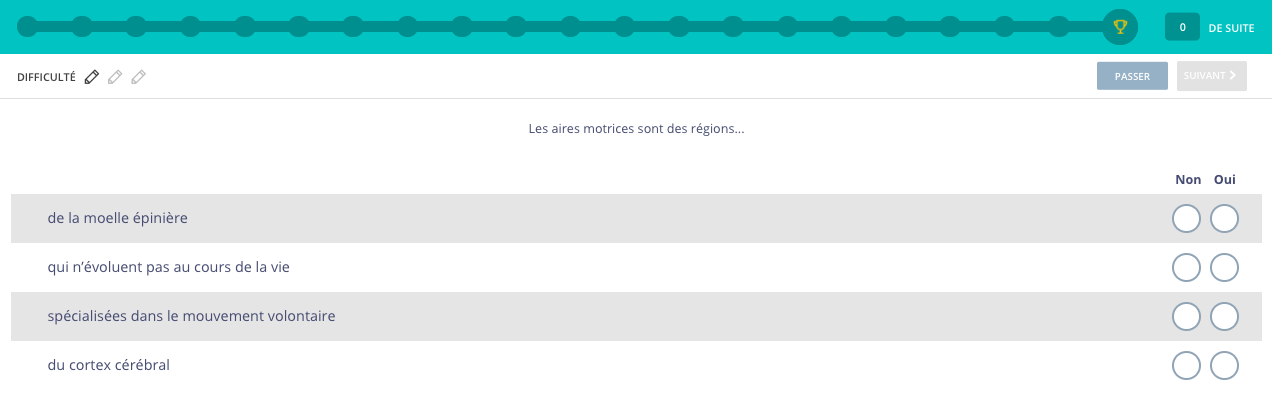
\includegraphics[clip, width= \textwidth]{1literature/fig/qcm.png}
\caption{"Multiple choice" is a question with several propositions which can be either true or false. }
\label{fig:qcm}
\end{figure*}

\begin{figure*}[!ht]
\centering
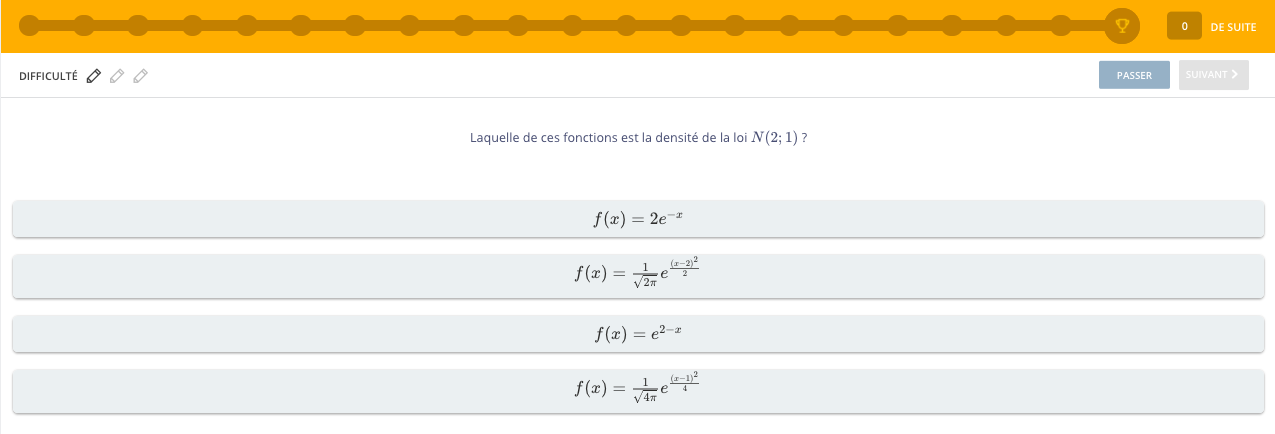
\includegraphics[clip, width= \textwidth]{1literature/fig/qcu.png}
\caption{The "single choice" is a question with several propositions (mostly, 2 or 4) and only one good answer.}
\label{fig:qcu}
\end{figure*}

\begin{figure*}[!ht]
\centering
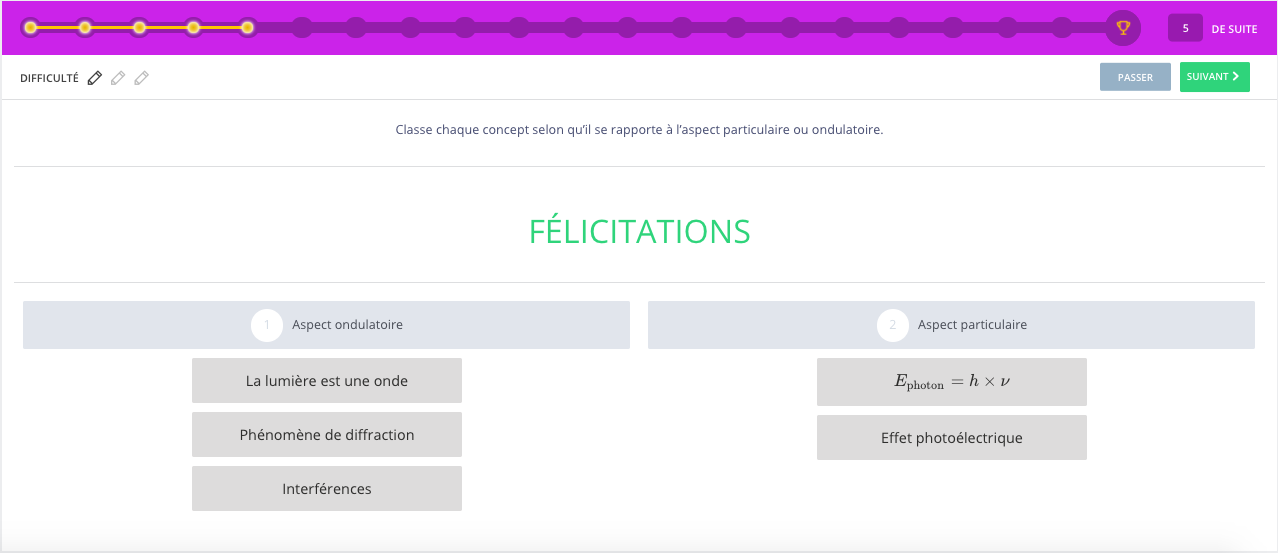
\includegraphics[clip, width= \textwidth]{1literature/fig/box.png}
\caption{"Box" is a type of exercises in which the student should sort several elements (e.g. 5) between two categories ("boxes").}
\label{fig:box}
\end{figure*}

\begin{figure*}[!ht]
\centering
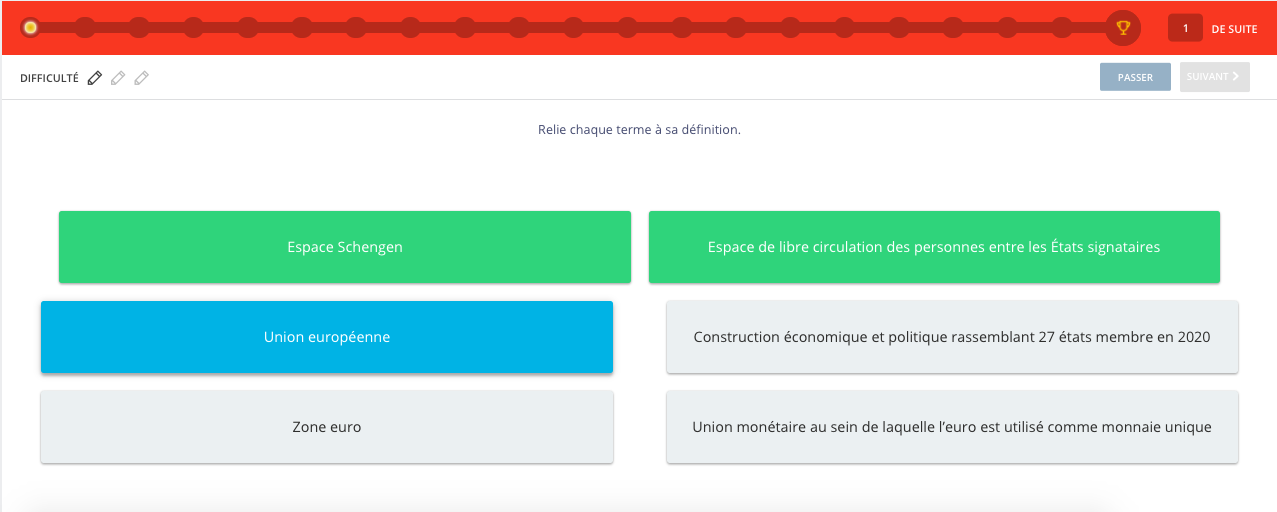
\includegraphics[clip, width= \textwidth]{1literature/fig/link.png}
\caption{"Link" exercises consist in linking each element of two different sets.}
\label{fig:link}
\end{figure*}

\begin{figure*}[!ht]
\centering
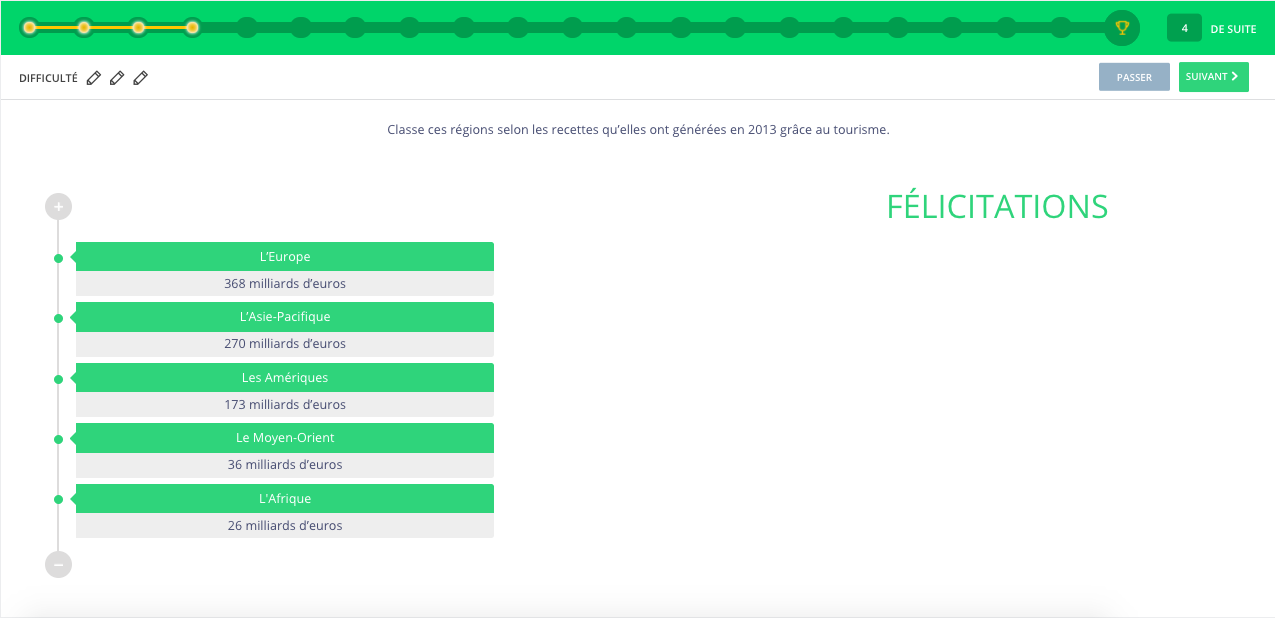
\includegraphics[clip, width= \textwidth]{1literature/fig/timeline.png}
\caption{A "timeline" consists in ordering different elements. It can be some dates in history,  but it can be used for any kind of ordered sets.}
\label{fig:timeline}
\end{figure*}

\begin{figure*}[ht]
\centering
\includegraphics[clip, width= \textwidth]{1literature/fig/input.png}
\caption{"Input" is a question with one or several blank holes that the learner should fill. }
\label{fig:input}
\end{figure*}

\clearpage
\section{Scope of the Ph.D.: how to choose the next exercise?}
The goal of this Ph.D. is to improve the way we choose the sequence of questions. In particular, we would like to select the next question in an adaptive way. It means that we would like to ask different questions to students depending on their respective estimated proficiency. 

There is a two-in-one objective: we would like to (1) accurately estimate the proficiency in order to (2) recommend more relevant questions. There is a trade-off to find between asking a question to measure the proficiency and asking a question because we think they are relevant. This problem is known in machine learning as the exploration-exploitation trade-off. In Chapter~\ref{ch:exploration}, we will present the main questions and answers the machine learning community brings to the topic of active exploration-exploitation.

In Chapter~\ref{ch:its}, we present the main gaps and limits of these general methods for application to educative systems. We also present other attempts to use these methods in adaptive educational systems.

The next three Chapters (\ref{ch:rested}, \ref{ch:restless}, and \ref{ch:pomdp}) are dedicated to the specific bandits problems we consider in this thesis.

\section{Users and usages}
Afterclasse content (both exercises and sheets) is free to use. A premium version is available with convenient tools: a printing option for the sheets, a revision planning to help the student organizing its exam revision on several days, etc. Because the content is free, it is very used nationwide: every year, tens of thousands of students complete several millions of exercises.

In June, there is a peak in the usage before the middle school (\emph{brevet des collèges}) and high school (\emph{baccalaur\'eat}) exams (Figure~\ref{fig:usage}). The number of active students in June is multiplied by three compared to the month of October. The total number of exercises is also multiplied by more than six, which shows that the average student is also doing twice more exercises in June than in October.  

\begin{figure*}[!ht]
\centering
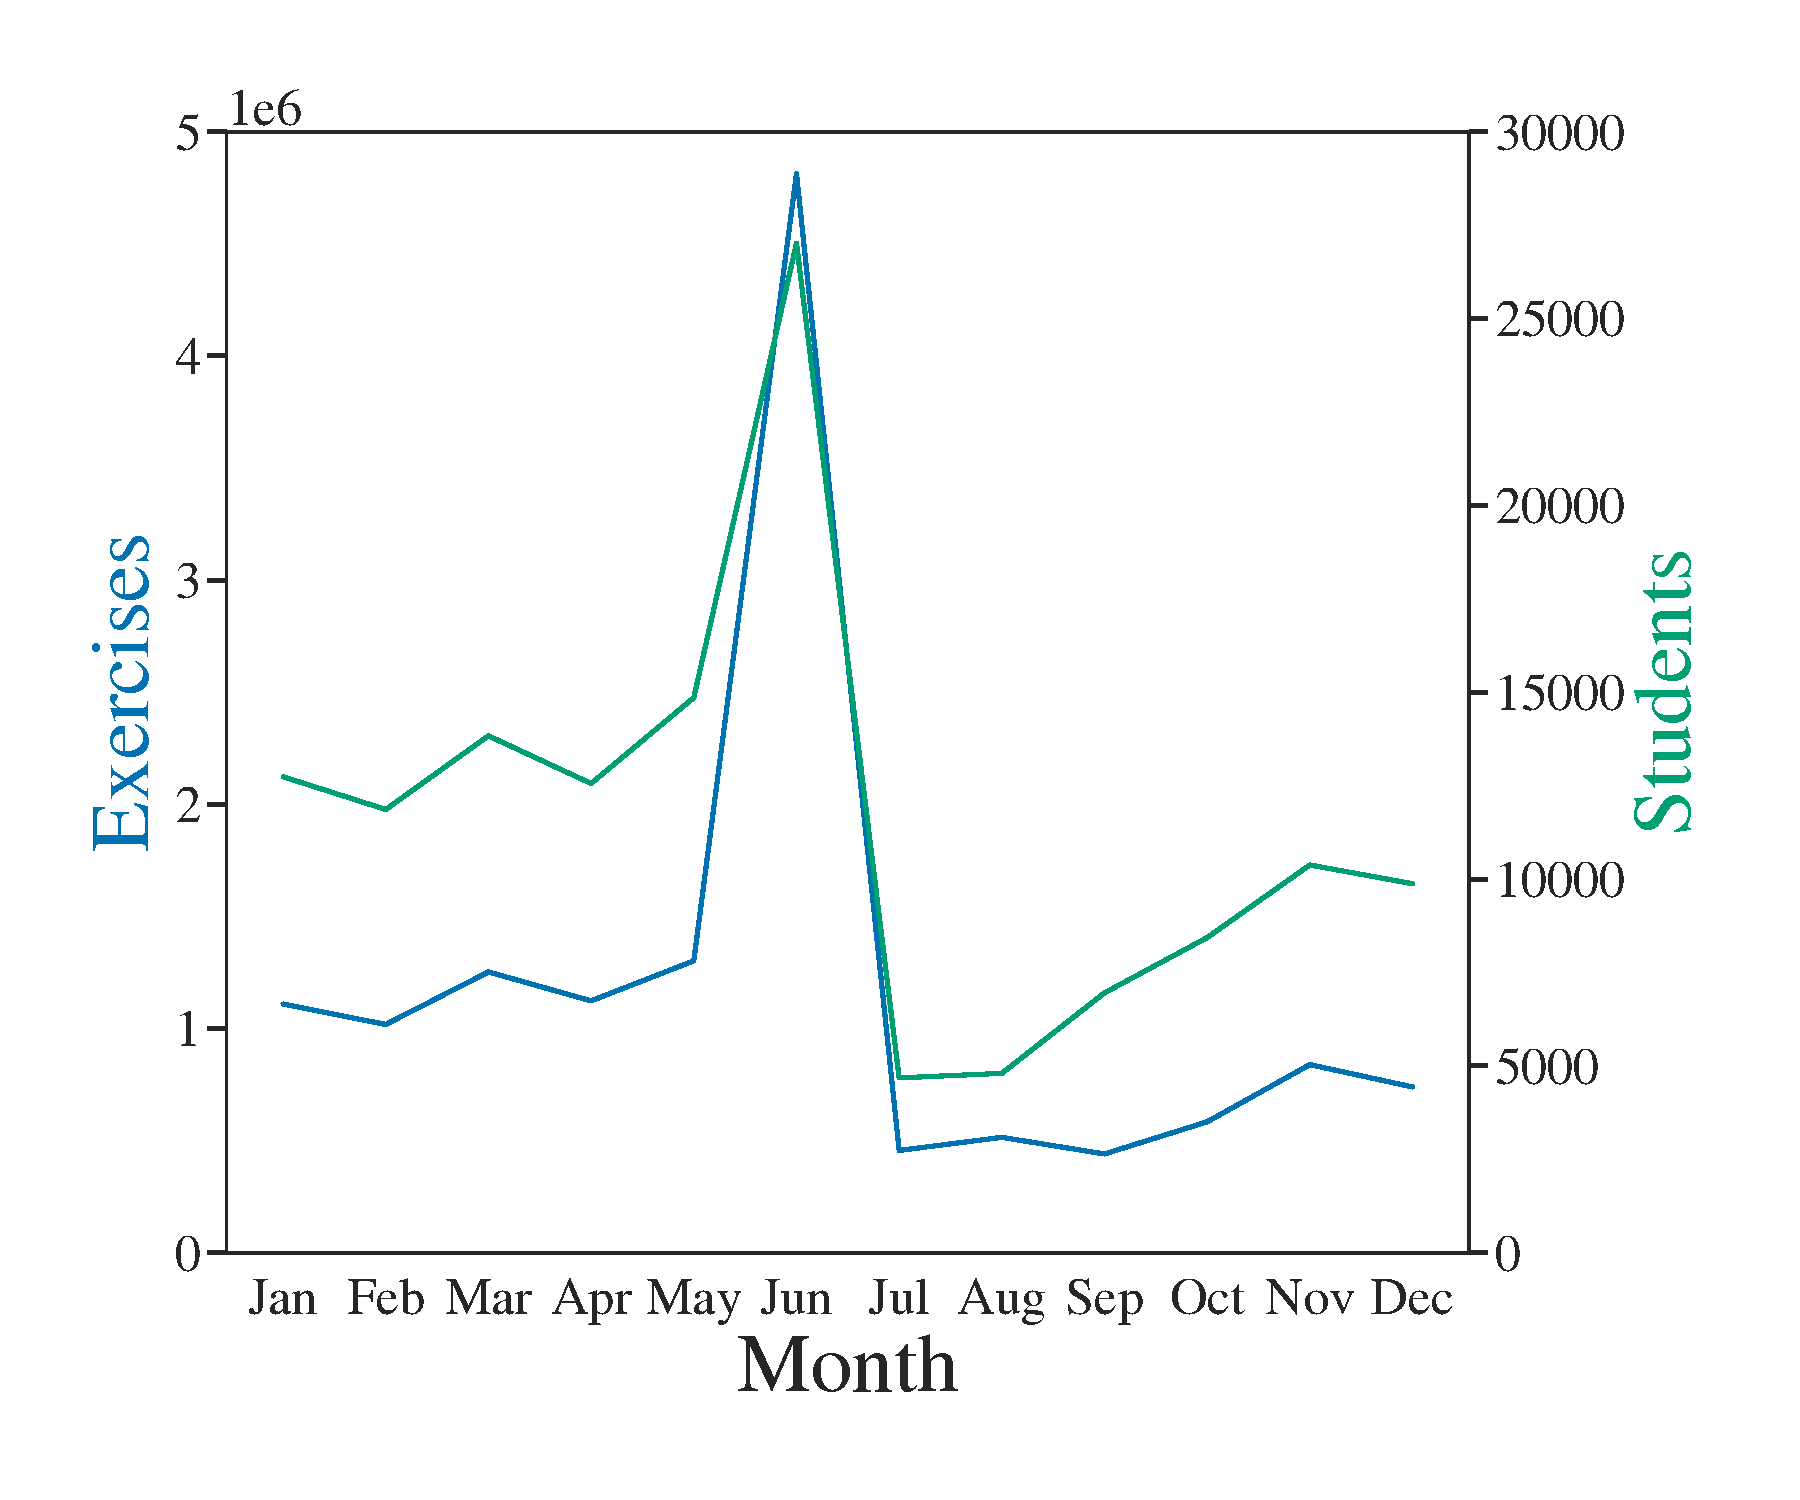
\includegraphics[clip, width= 0.75\textwidth]{1literature/fig/student-exercise.pdf}
\caption{Active logged-in students and their exercises per month} %TODO \footnote{the website can be used without registering. However, we have less information about these users.}
\label{fig:usage}
\end{figure*}

However, studying is not an addictive behavior and we notice a rather high churn rate (Figure~\ref{fig:churn}). Almost half of the logged-in students do not connect more than once to the website. After the first connection, we still loose a large fraction of the students between two connections. This fraction decreases to reach $10\%$ asymptotically. The fact that the churn rate converges to a positive number means that the number of students connecting at least $n$ times decreases exponentially with $n$. 

\begin{figure*}[!ht]
\centering
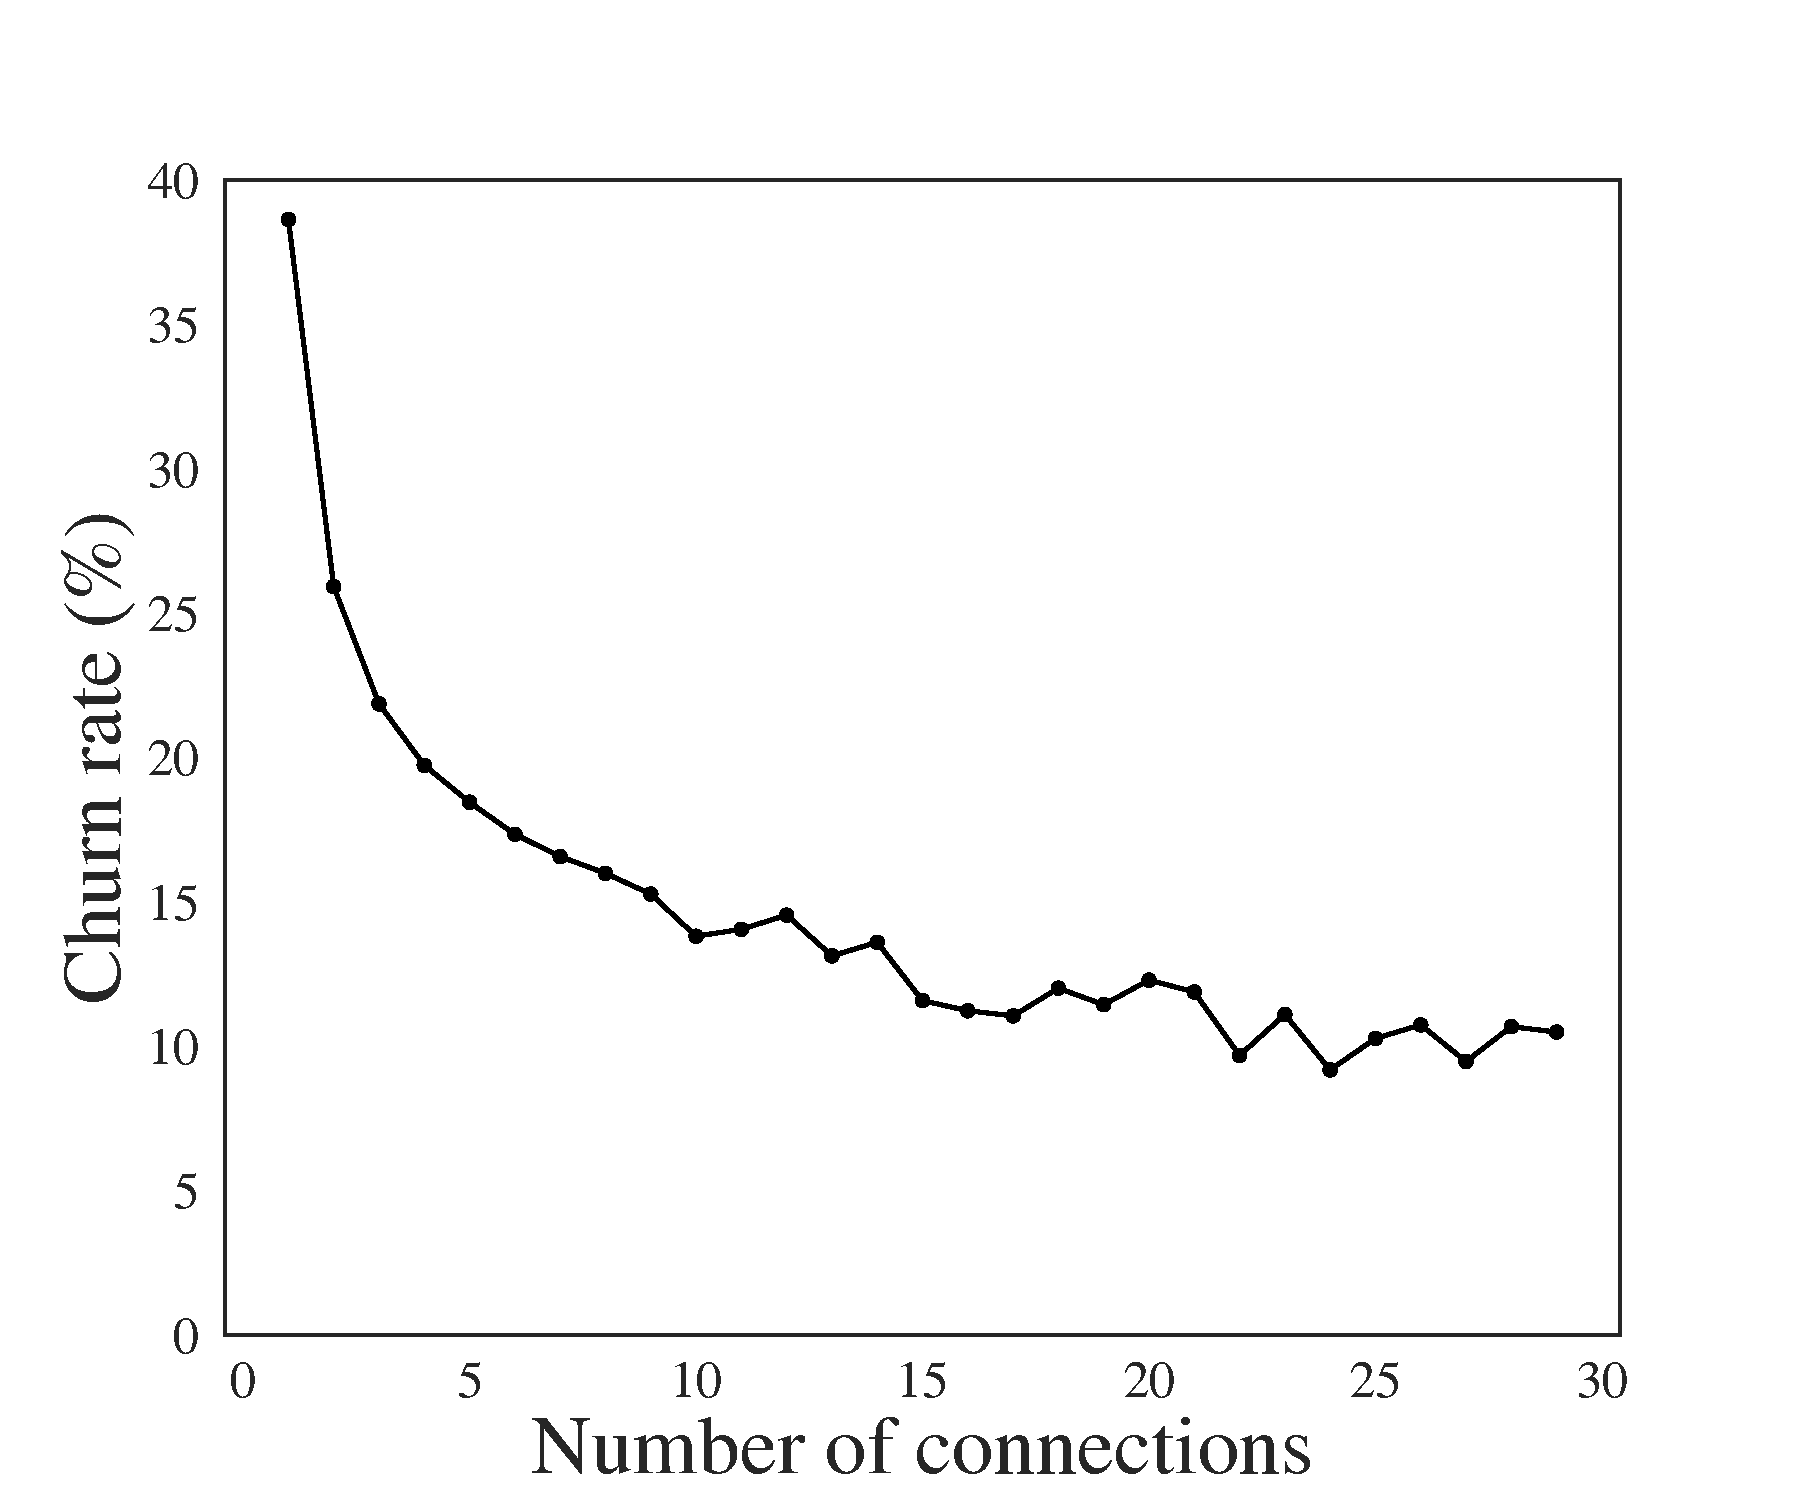
\includegraphics[clip, width= 0.75\textwidth]{1literature/fig/churn.pdf}
\caption{The churn rate is the proportion of students which do not connect $n+1$ times among the ones which connect $n$ times.}
\label{fig:churn}
\end{figure*}

Most of the students revise only one chapter per logged-in day. The repartition changes significantly just before the exams: half of the students revise 7 chapters per week or more in June while they are only $10\%$ in January. 

In brief, the students are cramming on the website: their revisions are short-term, intensive, and targeted (except during the final exams period in which they are broader). Due to the lack of long-term usage (and data), we will not address long-term objectives such as improving memory retention. Our upcoming approaches will focus on pragmatic short-term objectives: what are the gaps of the student \emph{now} and how can we fill them.


\section{Appendix: contextual elements on Lelivrescolaire.fr}
\label{sec:lls}
\href{https://www.lelivrescolaire.fr}{Lelivrescolaire.fr}\footnote{"le livre scolaire" means "the school textbook".} Editions (or lelivrescolaire.fr) publishes since 2010 educative contents and technologies for the French market. Within a few years, the company became one of the main actors of the national education ecosystem by gathering double expertise: strong publishing know-how and the ability to develop innovative technologies. 

Lelivrescolaire.fr brings up three key elements to distinguish themselves from other textbooks publishers. First, they promote free usage of their digital content. Indeed, each textbook's content is available for free on the website (\href{https://www.lelivrescolaire.fr}{www.lelivrescolaire.fr}), which is a unique fact in the French textbook publishing ecosystem. There are more than 2 million visitors each month on the website, which makes their digital textbooks the most used educative digital resources in France. 

Second, they write their educative content in a collaborative way. Lelivrescolaire.fr associates more than 100 teachers to the conception of each textbook. In total, it is more than 3000 teachers who have participated in middle school and high school textbooks conception for the last 4 years. 

Third, the company promotes constant innovation in the contents and digital media. Each textbook is available on the website and in desktop and tablet Apps. Moreover, the company released many features to enhance digital textbooks experience such as an embedded Python console for the programming exercises, an audio recorder for language learning, or multiple embedded tools for the science curriculum.  

More than half of the teachers and one million students in France are using digital content from Lelivrescolaire.fr. For printed books, Lelivrescolaire.fr represents more than 16\% of the market for many textbooks, which makes the company one of the leading actors in the French textbook publishing sector. The firm employs 50 workers dispatched in the technology division (engineers, developers, designers), the publishing division (publishers, graphic designers, community managers), and the customer support division (instructors, technical assistant). In January 2020, Lelivrescolaire.fr joined Hachette Livre, the third publishing company in the world.
